% !TeX root = ../index.tex
\documentclass[../index.tex]{subfiles}

\begin{document}
    \section{Wykład}
        Słońca także wykazuje charakterystyki typowe dla gwiazdy zmiennej, ale w jego przypadku wiąże się to z ewolucją pola magnetycznego (Słońca jest \textbf{aktywne magnetycznie}). Aktywnych w ten sposób gwiazd na ciągu jest bardzo dużo, tyczy się to m. in. karłów o typach K, G, F, M. Zjawiska związane z aktywnością magnetyczną Słońca, mogą wpływać na Ziemię – \textbf{pogoda kosmiczna}.\\
        Najbardziej znanym przejawem aktywności są \textbf{plamy słoneczne}:
        \begin{center}
            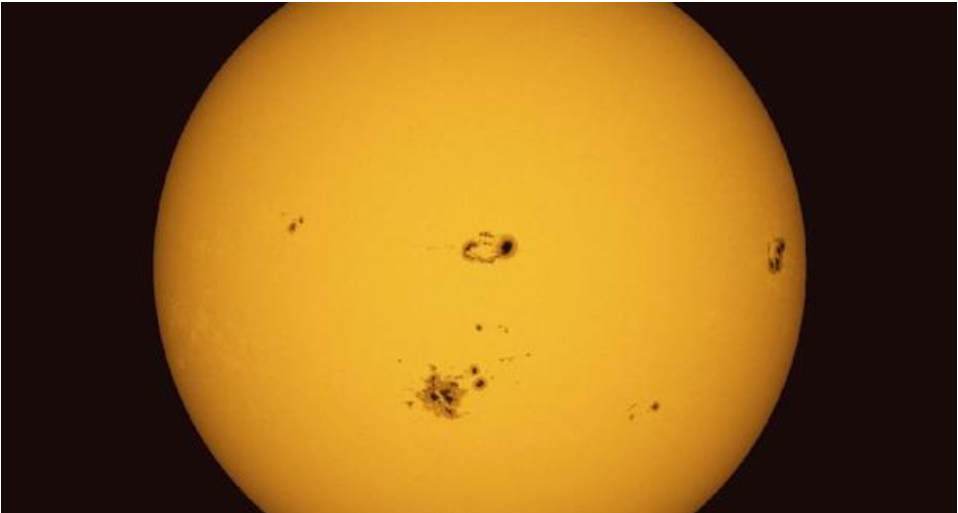
\includegraphics[width=13cm]{images/plamaSloneczna.png}
        \end{center}
        Dobrze ukształtowana plama składa się z \textbf{cienia} otoczonego \textbf{półcieniem} złożonym z radialnie ułożonych włókien:
        \begin{center}
            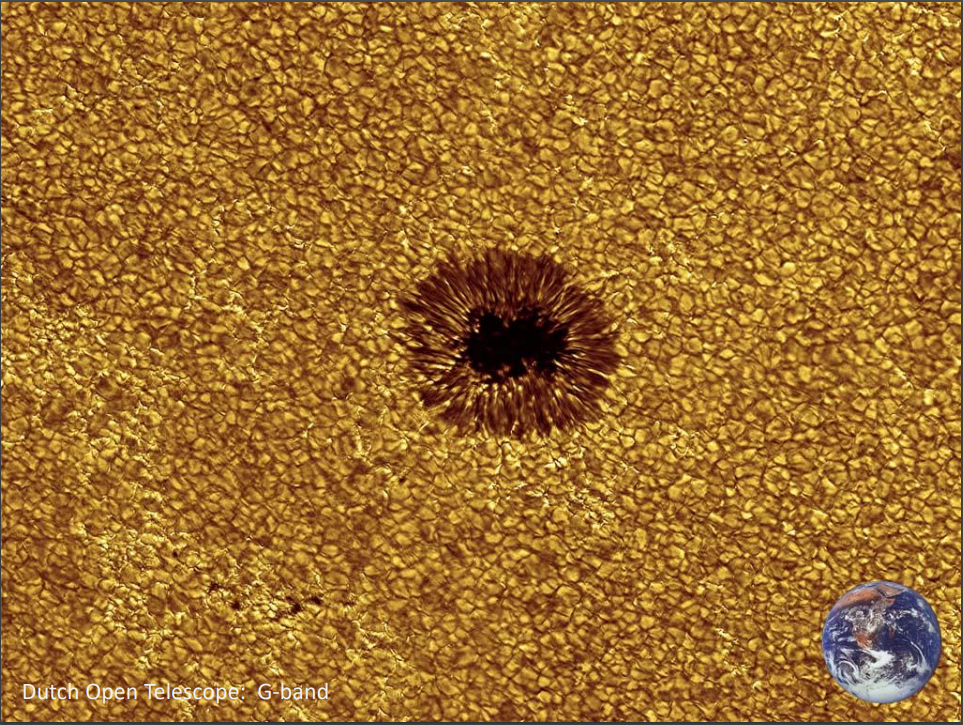
\includegraphics[width=13cm]{images/plamaSloneczna2.png}
        \end{center}
        Plama wydaje się ciemna ze względu na relatywnie niższą temperaturę względem reszty fotosfery: 200-300 K dla półcienia i 1500-2000 K dla cienia. Plamy często grupują się w \textbf{obszary aktywne}. Oprócz plam do obszarów zalicza się też okoliczne pojaśnienia zwane \textbf{polami pochodni}. Czas życia obszarów aktywnych może wynieść nawet kilka miesięcy.\\
        W aktywności słońca (pojawianiu się plam słonecznych) można zauważyć 11-letni cykl. W minimum często przez kilka miesięcy plamy nie pojawiają się w ogóle, a w maksimum ich liczba może przekroczyć 200. Nie jest to jednak bardzo regularny cykl i możliwe są nawet kilkudziesięcioletnie okresy, gdy plam się praktycznie nie obserwuje np. \textbf{minimum Maundera}. Plamy zajmują głównie obszary okołorównikowe, a ich szerokość heliograficzna maleje wraz z fazą cyklu (jak minium to blisko równika, jak maksimum to dalej). Plamy są lokalnymi koncentracjami pola magnetycznego. Odkrył to George Hale wykorzystując \textbf{efekt Zeemana}. Precyzyjne pomiary plam pozwalają odtworzyć linie pola magnetycznego Słońca – przypominają nie co fontannę: 
        \begin{center}
            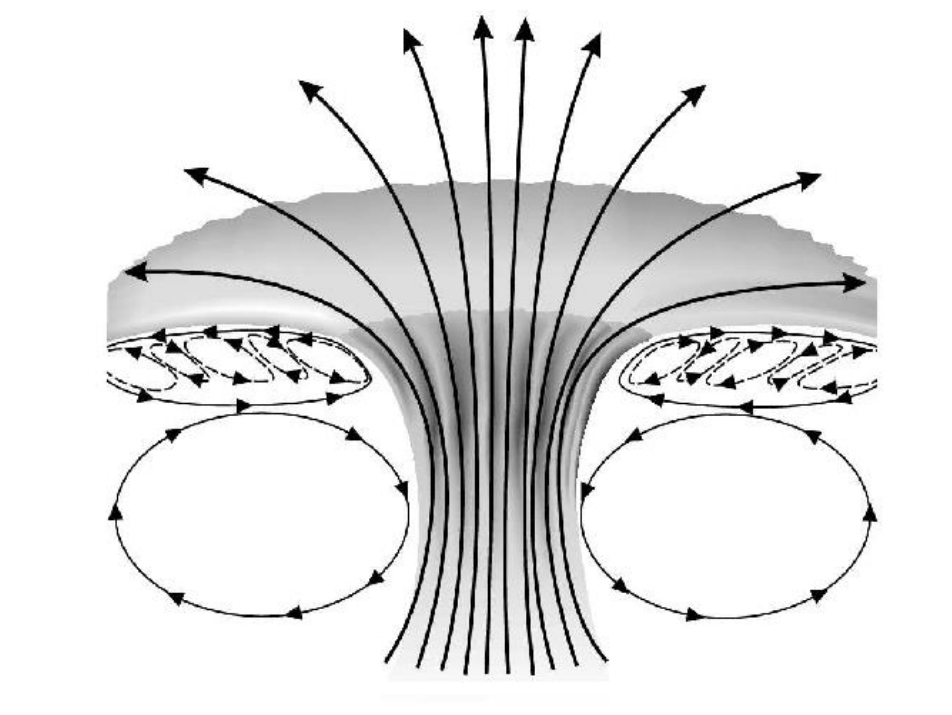
\includegraphics[width=13cm]{images/plamaSlonecznaFontanna.png}
        \end{center}
        Wiązki linii pola, uformowana i ściśnięta przez ruchy konwektywne, przebija się przez podstawę fotosfery i rozprzestrzenia na zewnątrz we wszystkich kierunkach. Obecność silnego pola ogranicza możliwość konwekcji, z czego wynika niższa temperatura w obrębie plamy.\\
        Pole magnetyczne jest generowane (dynamo) przez dwa rodzaju ruchów plazmy. Jeden z nich to ruchy konwektywne, a drugi, związany z rotacją słońca, to \textbf{rotacja różnicowa} – rotacja, która odbywa się z największą prędkością kątową na równiku, a z najmniejszą na biegunach. Taką rotacją objęta jest cała warstwa konwektywna, a szczególną rolę w generowaniu pola magnetycznego gra jej podstawa – \textbf{tachoklina}. W skrócie działanie \textbf{dynama słonecznego można opisać}:
        \begin{itemize}
            \item Dipolowy charakter globalnego pola magnetycznego (czyli taki jak w zwykłym magnesie) w minimum aktywności zmienia się na skutek rotacji różnicowej (a). Linie pola ,,wmrażane'' są w plazmę, w wyniku czego składowa poloidalna ulega rozciągnięciu i stopniowa zmienia się w składową toroidalną (b).
            \begin{center}
                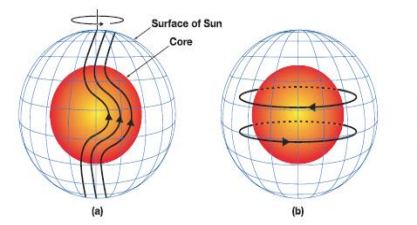
\includegraphics[width=8cm]{images/dynamoSloneczne1.png}
            \end{center}
            \item Ruchy konwektywne i siły Coriolisa dzielą globalne pole na mniejsze elementy, które wydostają się na zewnątrz (dzięki pływalności magnetycznej – cokolwiek to jest) i tworzą obszary aktywne (d, e, f)
            \begin{center}
                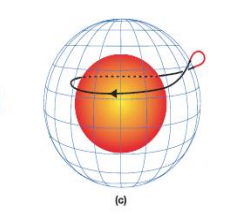
\includegraphics[width=4cm]{images/dynamoSloneczne2.png}
                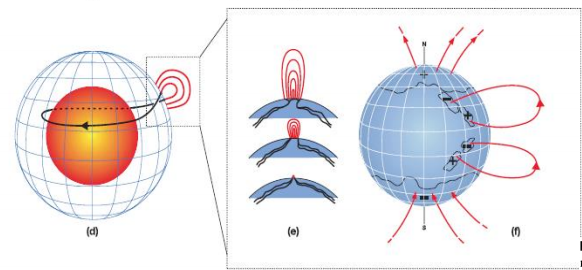
\includegraphics[width=9cm]{images/dynamoSloneczne3.png}
            \end{center}
            \item Pole magnetyczne obszarów aktywnych stopniowo upraszcza się i słabnie w wyniku m. in. anihilacji i dyfuzji (g).
            \begin{center}
                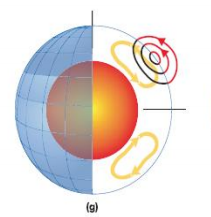
\includegraphics[width=4cm]{images/dynamoSloneczne4.png}
            \end{center}
            \item W wyniku rotacji pozostałości po obszarach aktywnych wędrują w kierunku biegunów (ruchu południkowe) wywołując w okolicach maksimum aktywności zmianę polaryzacji globalnego pola magnetycznego (h).
            \begin{center}
                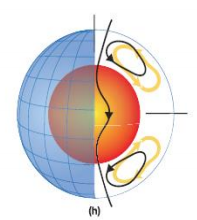
\includegraphics[width=4cm]{images/dynamoSloneczne5.png}
            \end{center}
            \item W następnym minimum odtworzona globalna składowa poloidalna ma przeciwny zwrot (f).
            \begin{center}
                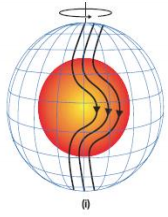
\includegraphics[width=4cm]{images/dynamoSloneczne6.png}
            \end{center}
        \end{itemize}
        Linie pola magnetycznego Słońca sięgają daleko w przestrzeń kosmiczną. Mają oną szczególną rolę w zewnętrznej warstwie atmosfery – \textbf{koronie słonecznej}, gdzie jakikolwiek ruch plazmy odbywać się może tylko wzdłuż linii pola.
        \begin{center}
            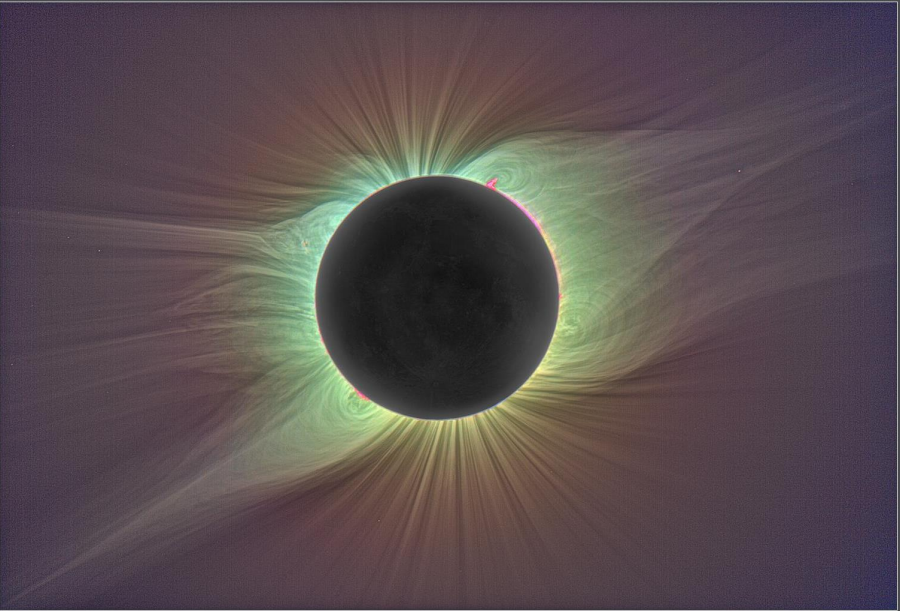
\includegraphics[width=13cm]{images/koronaSloneczna.png}
        \end{center}
        Korona jest rozrzedzona, ale przeniknięta silnym polem magnetycznym i łatwo przejmuje część jego energii – nagrzewa się do temperatur 0.7-2.5 mln K, a w obszarach aktywnych nawet do 6-8 mln K. Oznacza to emisje o w zakresie promieniowania X, które jest używane do obserwowania zjawisk w tym obszarze. Korzystając z tych obserwacji można odtwarzać linie pola magnetycznego w tej części atmosfery. Do wymienionych zjawisk należą m. in. \textbf{rozbłyski słoneczne} i \textbf{wielkoskalowe wyrzuty koronalne}.\\
        Rozbłyski słoneczne to nagłe i przejściowe pojaśnienia niewielkiego fragmentu słońca, spowodowane anihilacją pola magnetycznego w koronie. Są bardzo różnorodne i w zależności od wydzielonej energii oraz rozmiarów struktury magnetycznej mogą trwać od kilkunastu minut do kilkunastu godzin. Wielkość pojaśnienia zależy od długości fali. Np. w zakresie promieniowania X rozbłysk może zwiększyć jasność całej korony o kilka rzędów wielkości. Tak drastyczne zmiany są spowodowane wypełnianiem całej struktury magnetycznej korony przez gęstą plazmą chromosferyczną, która zostaje nagrzana do 25-40 mln. K. Rozbłyski pojawiają się wtedy, gdy w fotosferze obserwuje się plamy.\\
        W przypadku wielkoskalowych wyrzutów koronalnych (CME) energia zgromadzona w polu magnetycznym przekształcana jest na energię mechaniczną plazmy odrzuconej w przestrzeń międzyplanetarną. Wyrzut może propagować się z prędkością 1-2 tys. \(\frac{km}{s}\). Gdy chmura plazmy zostanie wypuszczona w kierunku Ziemi mówimy wówczas o \textbf{CME typu halo}. W chwili wniknięcia w ziemską magnetosferę, ruch cząstek odbywa się wzdłuż linii ziemskiego pola magnetycznego. Na pewnej odległości od biegunów magnetycznych oddziałując z cząstkami atmosfery tworzą \textbf{zorzę polarną}.\\
        Od lat 60. XX w. obserwuje się aktywność magnetyczną na innych gwiazdach. Duże zasługi w tej dziedzinie ma \textbf{Kosmiczny Teleskop Keplera} – orbitalny teleskop. Można obserwować zarówno cykliczne zmiany blasku (tzw. \textbf{fala fotometryczna}), nieregularne pojaśnienie (rozbłyski) jak i bezpośrednio korony gwiazdowe. Istnieją gwiazdy potrafiące generować rozbłyski o kilka rzędów wielkości silniejsze niż Słońce, ponieważ kluczowym parametrem jest prędkość rotacji gwiazdy, która spada z wiekiem, a Słońce do najmłodszych gwiazd nie należy (4.5 mld. lat).
\end{document}